\documentclass{standalone}
\usepackage{gravimeter,particles}
\usetikzlibrary{backgrounds}
\begin{document}
  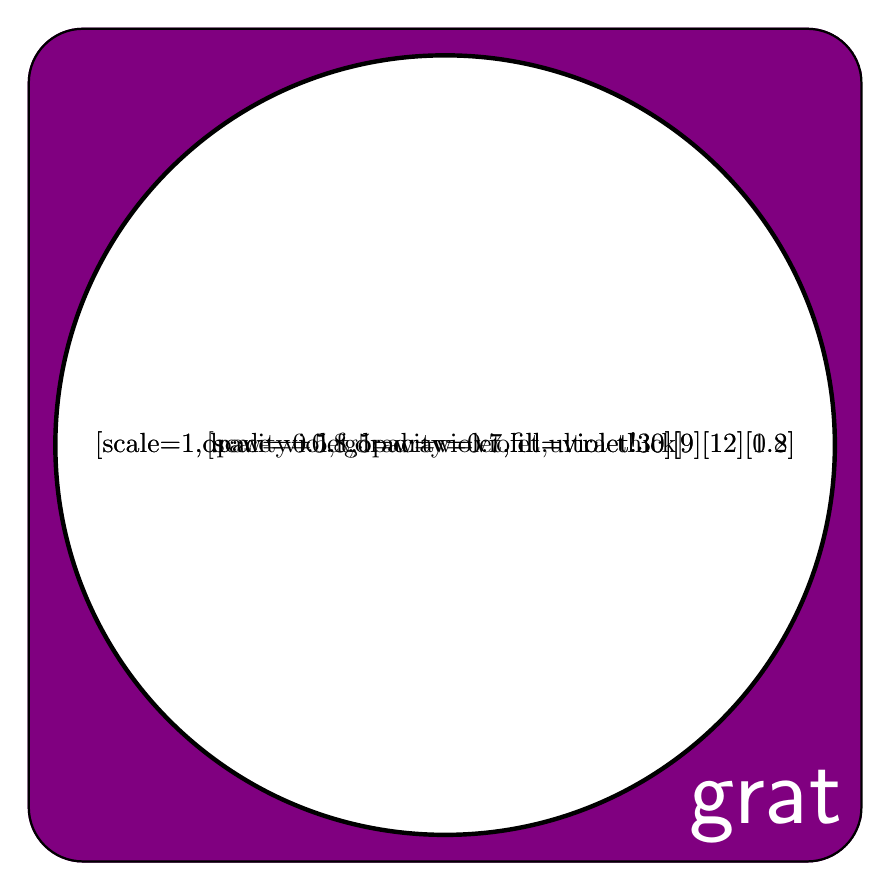
\begin{tikzpicture}
    \def\radius{4.95cm}
  \pdfsetrandomseed11
  \clip[rounded corners=2em]
    (-\radius-1em,-\radius-1em)
    rectangle
    (\radius+1em,\radius+1em)
    ; 
    \node{\particles[scale=1,opacity=0.8,draw=violet,fill=violet!30][9][12][1.2]};
    \node{
      \gravimeter[scale=0.5,fg5={draw=violet,ultra thick}]%
    };
    \node{\particles[scale=1,draw=violet,opacity=0.7,fill=violet!30][9][12][0.8]};
    \draw[
   ultra thick,
    violet,fill=violet, opacity=1,even odd rule,
    rounded corners=2em,
    draw=black
    ]
    circle(\radius)
    (-\radius-1em,-\radius-1em)
    rectangle 
    (\radius+1em,\radius+1em)
    ; 
    \node
    [
    anchor=south east,
    scale=1.4,
    font=\Huge\sffamily,
    outer sep=0.2em
    ]
    at(\radius+1em,-\radius-1em)
    {\color{white}grat}
    ;
    
   
  \end{tikzpicture}
\end{document}
